\documentclass[a4paper,twoside]{article}
\usepackage{graphicx} 
\usepackage{epstopdf}
\usepackage{epsfig}
\usepackage{subfigure}
\usepackage{calc}
\usepackage{amssymb}
\usepackage{amstext}
\usepackage{amsmath}
\usepackage{amsthm}
\usepackage{lscape}
\usepackage{multicol}
\usepackage{pslatex}
\usepackage{apalike}
\usepackage{SCITEPRESS}
\usepackage[small]{caption}
\usepackage{algorithm}
\usepackage{algorithmic}
\usepackage{enumerate}
\renewcommand{\algorithmicrequire}{\textbf{Input:}}
\renewcommand{\algorithmicensure}{\textbf{Output:}}
\def\R{{\mathbb R }}
\def\N{{\mathbb N }}
\subfigtopskip=0pt
\subfigcapskip=0pt
\subfigbottomskip=0pt
\begin{document}

\title{An Online Vector Error Correction Model for Exchange Rates Forecasting}


\author{\authorname{Paola Arce\sup{1}, Jonathan Antognini\sup{1}, Werner
Kristjanpoller\sup{2} and Luis Salinas\sup{1,3}}
\affiliation{\sup{1}Departamento de Inform\'atica, Universidad T\'ecnica Federico
Santa Mar\'ia, Valpara\'iso, Chile}
\affiliation{\sup{2}Departamento de Industrias, Universidad T\'ecnica Federico
Santa Mar\'ia, Valpara\'iso, Chile}
\affiliation{\sup{3}CCTVal, Universidad T\'ecnica Federico
Santa Mar\'ia, Valpara\'iso, Chile}
\email{\{paola.arce,luis.salinas,werner.kristjanpoller\}@usm.cl, jantogni@csrg.inf.utfsm.cl}
}

\keywords{Vector Error Correction Model, Online Learning, Financial
Forecasting, Foreign Exchange Market}

\abstract{
Financial time series are known for their non-stationary behaviour. However,
sometimes they exhibit some stationary linear combinations. When this happens,
it is said that those time series are cointegrated.The Vector Error Correction
Model (VECM) is an econometric model which characterizes the joint dynamic
behaviour of a set of cointegrated variables in terms of forces pulling towards
equilibrium. In this study, we propose an Online VEC model (OVECM) which
optimizes how model parameters are obtained using a sliding window of the most
recent data. Our proposal also takes advantage of the long-run relationship
between the time series in order to obtain improved execution times. Our
proposed method is tested using four foreign exchange rates with a frequency of
1-minute, all related to the USD currency base. OVECM is compared with VECM and
ARIMA models in terms of forecasting accuracy and execution times. We show that
OVECM outperforms ARIMA forecasting and enables execution time to
be reduced considerably while maintaining good accuracy levels compared with
VECM.
}

\onecolumn \maketitle \normalsize \vfill


\section{Introduction}
The learning from examples problem is an ill-posed problem which
admits an infinite number of solutions.  In order to restrict the
space of admissible solutions, the regression problem is usually
formulated in terms of regularization theory~\cite{girosiETal1995} as
an optimization problem, which minimizes the functional: 

\begin{equation}
\label{eq:problem} 
J(\mathbf{w}) = \sum_{t=1}^m (y_t - f(\mathbf{x}_t))^2 + \gamma R(\mathbf{w})
, \qquad f \in \mathcal{H} \, ,
\end{equation}

\noindent where $m$ is the number of samples $(\mathbf{x}_t ,y_t)$ with
$\mathbf{x}_t \in \R^l$, $l$ correspond to the number of features, $y_t
\in \R$ is the target, $R(\mathbf{w}) = ||w||^2$ where $||.||^2_K$ is a norm in a
{\em reproducing kernel hilbert space} $\mathcal{H}$ defined by the
positive definite form $K$, and $\gamma$ is a regularization
parameter~\cite{evgeniouETal2000}.
%Qué norma debe usarse? falta definir K
When the hypothesis space is reduced, the risk of overfitting the training data
decreases and therefore leading to better generalization capability. 
%aclarar porqué se reduce el espacio de hipótesis
{\em Ridge regression} (RR) is a batch method generally used to solve this
problem, which is a generalization of least squares method (LS). 

%RR is a batch method and it is not used in an online context mainly because
%it uses large amount of data and the number of operations increases
%with data size.

However, online algorithms are more attractive than batch algorithms because
their simplicity and ability to manage large data sets, this is why
they are popular in financial applications.

There are several popular online methods such as
perceptron~\cite{rosenblatt58},
passive-aggressive~\cite{crammerETall2006}, stochastic gradient
descent~\cite{zhang2004}, aggregating algorithm~\cite{vovk2001} and
the second order perceptron~\cite{cesa-bianchi2005}.
In~\cite{cesa-bianchi2006} it is provided an in-deph analysis of
online learning.

The {\em aggregating algorithm for regression} (AAR) method formulates
a recursive formulation of RR in an online way. AAR
consider all data to make a prediction, but in highly variant
scenarios the old data could be useless.

In this paper, we propose an online method based on the idea presented
by~\cite{vovk2001} considering in our case a single sliding window of
the most recent data. This proposal also reduces the number of
operations at every step of the algorithm by expressing the inverse
matrix in an iterative form. Our algorithm is later tested with
financial data from stock market.



\def\rot#1{{\color{red}{#1}}}
\def\gruen#1{{\color{green}{#1}}}
\def\blau#1{{\color{blue}{#1}}}


\section{\uppercase{Background}}
\label{sec:background}

\subsection{Integration and Cointegration}\label{sec:coint}\  
Following Johansen \cite{johansen1995} we shall say that a stochastic process
$Y_t$ which satisfies $Y_t-E(Y_t) = \sum_{i=0}^\infty C_i\,\varepsilon_{t-i}$ is
called $I(0)$, and then we shall write $Y_t\sim I(0)$, whenever
$\sum_{i=0}^\infty C_i \neq 0$ and $\sum_{i=0}^\infty C_i\,z^i$ converges for
$z\in\mathbb{C}$ with $|z|<1$.  It is understood that the condition
$\varepsilon_t\sim iid(0,\sigma^2)$ holds.

A (vector) time series $\mathbf{y}_t$ is said to be {\em integrated of order\/}
$d$, and then we shall write $\mathbf{y}_t\sim I(d)$, whenever after $d$ times
(discrete) differentiation an stationary process is obtained~\cite{banerjee1993};
more precisely, whenever
$(1-L)^d\,\mathbf{y}_t\sim\text{I(0)}$, where $L$ is the usual lag operator:
$(1-L)\,\mathbf{y}_t = \Delta\mathbf{y}_t = \mathbf{y}_t-\mathbf{y}_{t-1}$ for
all $t$.  

Note that this definition includes the scalar case as time series of
vectors of dimension 1; in this scalar case we will write the time series in
nonbold format.

Let $\mathbf{y}_t^\nu$, $\nu=1,\dots,l$, be a set of $l$ vector time series of
order $I(1)$.  They are said to be {\em cointegrated\/} if a vector
$\beta=[\beta(1),\dots,\beta(l)]^\top \in \mathbb{R}^p$ exists, such that the
time series,
\begin{equation}
\mathbf{Z}_t:= 
\sum_{\nu=1}^l \beta(\nu)\,\mathbf{y}_t^\nu\,\sim\,\text{I(0)}\,.
\end{equation}
In other words, a set of $I(1)$ time series is said to be cointegrated if a
linear combination of them exists, which is I(0).


\subsection{Vector Autorregresive Models}\label{sec:varvec}

Vector error correction model (VECM) describe the joint behaviour
of a set of variables and can be derived from the simple Vector Autoregressive model (VAR) \cite{sims1980} model.
The VAR($p$) model is a framework describing the behaviour of a
set of $l$ endogenous and stationary variables as a linear combination of their last $p$
values, where $l,p\in\mathbb{N}$. 
In our case, each one of these $l$ variables is a scalar time series
$y_{\lambda,t}$, $\lambda=1,\dots,l$, and we represent them all together
at time $t$ by the the vector time series:
\begin{equation}
\label{eq:variables}
\mathbf{y}_t = 
\begin{bmatrix} y_{1,t} & y_{2,t} & \dots & y_{l,t} \end{bmatrix}^\top.
\end{equation}
\noindent
Notice that the vectors $\mathbf{y}_t$ are assumed to be $l$-dimensional.

The VAR($p$) model describes the behaviour of a dependent variable in terms of
its own lagged values and the lags of the others variables in the system. The
model with $p$ lags is formulated as the system of $N$:
\begin{align}
\label{eq:var}
\mathbf{y}_t 
= \boldsymbol{\Phi}_1 \mathbf{y}_{t-1} +
  \boldsymbol{\Phi}_2 \mathbf{y}_{t-2} + \dots +
  \boldsymbol{\Phi}_p\mathbf{y}_{t-p} +
  \mathbf{c} + \boldsymbol{\epsilon}_t \nonumber \\
t=p+1,\dots,N,
\end{align}
\noindent where 
$\boldsymbol{\Phi}_1, \boldsymbol{\Phi}_2,\dots,\boldsymbol{\Phi}_p$
are $l\times l$-matrices of real coefficients,
$\boldsymbol{\epsilon}_{p+1},
 \boldsymbol{\epsilon}_{p+2}, \dots, \boldsymbol{\epsilon}_N$ 
are error terms, $\mathbf{c}$ is a constant vector and $N$ is the total
number of samples.

Notice that, regarding our notation of section (\ref{sec:coint}),
we have here 
$\mathbf{y}_t^0 = \mathbf{y}_t$,
$\mathbf{y}_t^\nu = \mathbf{y}_{t-\nu}$ and
the $\lambda$-th component of the vector time series $\mathbf{y}_t^\nu$
is the scalar time series $y_{\lambda,t}^\nu$, where $\nu=1,\dots,p$ and
$\lambda=1,\dots,l$.

However, the VAR model cannot be used with non-stationary variables. VECM \cite{engle87} is also a linear model and a special form of a VAR model for I(1) variables that are also
cointegrated~\cite{banerjee1993}. If cointegration exists, variable differences
are stationary and they introduce an error correction term which adjusts
coefficients to bring the variables back to equilibrium. 


It is obtained re-writing equation (\ref{eq:var}) in terms of the new
variable $\Delta\mathbf{y}_t=\mathbf{y}_t-\mathbf{y}_{t-1}$.
The VECM model, expressed in terms those differences, takes the form:
\begin{equation}\label{eq:vec}
\Delta \mathbf{y}_t 
= \boldsymbol{\Omega}\,\mathbf{y}_{t-1}
  + \sum_{i=1}^{p-1} \boldsymbol{\Phi}_i^*\,\Delta\mathbf{y}_{t-i}
  + \mathbf{c} + \boldsymbol{\epsilon}_t\,,
\end{equation}
\noindent
where the coefficients matrices $\boldsymbol{\Phi}_i^*$ and 
$\boldsymbol{\Omega}$, expressed in terms of the matrices
$\boldsymbol{\Phi}_i$ of (\ref{eq:var}), are:
\begin{align*}
\boldsymbol{\Phi}_i^* 
&:= -\sum_{j=i+1}^{p}\boldsymbol{\Phi}_j\,, \\
\boldsymbol{\Omega}
&:= -\left( \mathbb{I} - \boldsymbol{\Phi}_1 - \dots 
    - \boldsymbol{\phi}_p \right)\,. 
\end{align*}
The following well known properties of the matrix $\boldsymbol{\Omega}$
\cite{johansen1995} will be useful in the sequel:
\begin{itemize}
\item
If $\boldsymbol{\Omega} = \mathbf{0}$, there is no cointegration.
\item 
If $rank(\boldsymbol{\Omega})=l$, i.e., if $\boldsymbol{\Omega}$ has
full rank, then the time series are not I(1) but stationary.
\item
If $rank(\boldsymbol{\Omega})=r$, $0<r<l$, then there is cointegration
and the matrix $\boldsymbol{\Omega}$ can be expressed as
$\boldsymbol{\Omega}=\boldsymbol{\alpha\beta}^\top$, where $\boldsymbol{\alpha}$
and $\boldsymbol{\beta}$ are
$l\times r$ matrices and
$\text{rank}(\boldsymbol{\alpha})=\text{rank}(\boldsymbol{\beta})=r$.
\item
The columns of $\boldsymbol{\beta}$ contains the cointegration vectors and the rows of
$\boldsymbol{\alpha}$ correspond with the adjusted vectors. 
$\boldsymbol{\beta}$ is obtained by Johansen procedure~\cite{johansen1988},
whereas $\boldsymbol{\alpha}$ has to be determined as a variable in the VECM.
\end{itemize}
It is worth noticing that the factorization of the matrix
$\boldsymbol\Omega$ is not unique, since for any $r \times r$
non-singular matrix $\mathbf{H}$, $\boldsymbol{\alpha}^*:=\boldsymbol{\alpha}\mathbf{H}$,
and $\boldsymbol{\beta}^*=\boldsymbol{\beta}(\mathbf{H}^{-1})^\top$ we have
$\boldsymbol{\alpha\beta}^\top=\boldsymbol{\alpha}^*(\boldsymbol{\beta}^*)^\top$.
If cointegration exists, then equation (\ref{eq:vec}) can be written
as follows:
\begin{equation}\label{eq:vecfull}
\Delta\mathbf{y}_t 
= \boldsymbol{\alpha\beta}^\top\mathbf{y}_{t-1} 
  + \sum_{i=1}^{p-1}\boldsymbol{\Phi}_i^*\,\Delta\mathbf{y}_{t-i}
  + \mathbf{c} + \boldsymbol{\epsilon}_t\,,
\end{equation}
\noindent
which is a VAR model but for time series differences.


Transposing each equation of the system (\ref{eq:vecfull}) we can write
the VECM($p$) model in block-matrix form as:
\begin{equation}\label{eq:vareq}
\mathbf{B} = 
\mathbf{A} \mathbf{X} + 
\mathbf{E} \, , 
\end{equation}
%
\noindent where $\mathbf{B}$ dimension is $((N-p)\times l)$, $\mathbf{A}$
dimension is $((N-p)\times(r+(p-1)l +1))$, $\mathbf{X}$ dimension is $((r+(p-1)l
+1)\times l)$ and $\mathbf{E}$ dimension is $((N-p)\times l)$:
%
\begin{alignat}{3}
\mathbf{B}
&= \begin{bmatrix}
   \Delta\mathbf{y}_{p+1}^\top \\
   \Delta\mathbf{y}_{p+2}^\top \\
   \vdots \\
   \Delta\mathbf{y}_N^\top
   \end{bmatrix}
&\quad
\mathbf{X}
&= \begin{bmatrix}
   \boldsymbol{\alpha}^\top \\
   \boldsymbol{\Phi}_1^{*\top} \\
   \boldsymbol{\Phi}_2^{*\top} \\
   \vdots \\
   \boldsymbol{\Phi}_{p-1}^{*\top} \\
   \mathbf{c}^\top
   \end{bmatrix}
&\quad
\mathbf{E}
&= \begin{bmatrix}
   \boldsymbol{\epsilon}_{p+1}^\top \\
   \boldsymbol{\epsilon}_{p+2}^\top \\
   \vdots \\
   \boldsymbol{\epsilon}_N^\top \\
   \end{bmatrix}
\end{alignat}
\noindent and 
\begin{align}
\mathbf{A} 
&= \begin{pmat}[{....|}]
   \mathbf{y}_p^\top \boldsymbol{\beta} & \Delta \mathbf{y}_p^\top & \Delta\mathbf{y}_{p-1}^\top & \dots 
                    & \Delta\mathbf{y}_2^\top & 1 \cr
   \mathbf{y}_{p+1}^\top  \boldsymbol{\beta} &\Delta\mathbf{y}_{p+1}^\top & \Delta\mathbf{y}_p^\top & \dots
                       & \Delta\mathbf{y}_3^\top & 1 \cr
   \vdots & \vdots & \vdots & \ddots & \vdots & \vdots \cr
   \mathbf{y}_{N-1}^\top  \boldsymbol{\beta} &\Delta\mathbf{y}_{N-1}^\top & \Delta\mathbf{y}_{N-2}^\top & \dots 
                       & \Delta\mathbf{y}_{N-p-1}^\top & 1 \cr
   \end{pmat}\, .
\label{eq:Amatrix}
\end{align}
Taking into account the error term $\mathbf{E}$, equation~(\ref{eq:vareq}) 
can be solved with respect to $\mathbf{X}$ using the ordinary least
squares (OLS) estimation.
\section{\uppercase{Methodology}}
\label{sec:methodology}
\noindent 
%\subsection{Online VECM} \label{sec:proposal}

Since financial problems are stream data problems, it is unfeasible to include
all input data in a VECM model. Our proposal consists on an online version of
VECM (OVECM) capable of updating the model with new arrival data and give
responses in a short period of time. OVECM only considers a time varying window
of historical data and the using of RR instead of OLS to get model parameters in
order to avoid sensitivity to input data errors.

On the other hand, getting cointegration vectors using Johansen method is also
an expensive procedure. However, since cointegration
vectors represent the long-run relationship between the time series, they
vary little in time. Our proposal obtains new cointegration vectors only when
this long-term relationship changes. This change is detected by tracking 
the Mean Absolute Percentage Error (MAPE) of the last $n$ in-sample forecasts.

Since VECM is a model based on time series differences, the MAPE is obtained
from $\Delta \mathbf{y}$ as following:
 
\begin{equation}\label{eq:MAPE}
\text{MAPE}[t] = \frac{1}{n} \sum_{i=1}^{n} \left| 
\frac{\Delta \mathbf{y}_{\text{true}}[t-i]-\Delta
\mathbf{y}_{\text{pred}}[t-i]}{\Delta \mathbf{y}_{\text{true}[t-i]}}
\right| \, , 
\end{equation}

\noindent where $\Delta \mathbf{y}_{\text{true}}$ is the actual value of the
time series $\mathbf{y}$ differences and $\Delta \mathbf{y}_{\text{pred}}$ is
their forecast value.




%The method proposed consists of
%a modification of RR considering a sliding window which contains only
%the last $L$ samples %and the new input $\mathbf{x}_t$, 
%i.e. $\{\mathbf{x}_i\}_{i=t-L+1}^{t-1}$. 

In order to formulate this algorithm we need to define first the
following matrices:
 
\begin{equation}
\label{eq:notation}
	\mathbf{A}(t) = 
\left[
  \begin{tabular}{c>{$}c<{$}c}
    --- & \mathbf{a}^{\top}_{t-L} & ---\\
    --- & \mathbf{a}^{\top}_{t-L+1} & ---\\
    & \vdots & \\
    --- & \mathbf{a}^{\top}_{t} & ---
  \end{tabular}
\right]
\quad \text{and} \quad
\mathbf{B} =
\left[
  \begin{tabular}{c>{$}c<{$}c}
    --- & \mathbf{b}_{t-L} & ---\\
    --- & \mathbf{b}_{t-L+1} & ---\\
    & \vdots & \\
    --- & \mathbf{b}_{t} & ---
  \end{tabular}
\right] \, ,
\
\end{equation}


The optimal solution using a sliding windows is then:

\begin{eqnarray}
\label{eq:optsolSLAAR}
\mathbf{X}(t)&=&({\bf A}(t)^\top{\bf A}(t)+
\gamma \mathbb{I})^{-1}{\bf A}(t)^\top{\bf B}(t) \\
\mathbf{X}(t)&=&\mathbf{S}(t)^{-1} \mathbf{W}(t) \, ,
\end{eqnarray}

\noindent where we can also write: 

\begin{eqnarray}
\mathbf{S}(t) =&{\bf A}(t)^\top{\bf A}(t)+ \gamma \mathbb{I} &=
\sum_{i=0}^L \mathbf{a}_{t-i}\mathbf{a}_{t-i}^\top + \gamma \mathbb{I}
\label{eq:S} \\
\mathbf{W}(t) =& {\bf A}(t)^\top{\bf B}(t) &= 
\sum_{i=0}^L \mathbf{a}_{t-i}\mathbf{b}_{t-i} 
\label{eq:W}
\end{eqnarray}

It is worth noticing that the matrices $\mathbf{S}(t+1)$ and $\mathbf{W}(t+1)$
are slightly different: 

\begin{eqnarray*}
\mathbf{S}(t+1)&=&
\mathbf{S}(t) +
\mathbf{a}_{t+1}
\mathbf{a}_{t+1}^\top -
\mathbf{a}_{t-L} \mathbf{a}_{t-L}^\top \\
\mathbf{W}(t+1)&=&
\mathbf{W}(t) +
\mathbf{a}_{t+1}
\mathbf{b}_{t+1} -
\mathbf{a}_{t-L} \mathbf{b}_{t-L} \, .
\end{eqnarray*}

Therefore Sherman-Morrison-Woodbury formula can be used to reduce inverse matrix
calculations.

The algorithm~\ref{alg:proposal} shows our online VECM using three different
methods for geting model parameters: OLS, RR, AAR.

\begin{algorithm}[ht]
\begin{algorithmic}[1]
\REQUIRE $\,$ \\
$\mathbf{y}$: matrix with $N$ input vectors and $l$ time series\\
$p$: number of past values \\
method: \{'OLS','RR','AAR'\} \\
$\lambda$: regularization parameter (only requires for RR and AAR methods) \\
$L$: window size of data($L<N$) \\
$\text{mean\_error}$: MAPE threshold \\
$n$: windows size to obtain in-sample MAPE \\
\ENSURE  $\,$ \\
$\{\mathbf{y}_{\text{pred}}[L+1],\dots, \mathbf{y}_{\text{pred}}[N]\}$: model predictions 
\STATE solver = new \texttt{Solver}(method,$\lambda$) \\
\FOR { $t =1$ to $N-L$ }
    \STATE $\mathbf{Y} \gets \mathbf{y}[t:t+L-1]$
    \STATE $\mathbf{y}_t \gets \mathbf{y}[t+L]$
	\IF {$t = 1$}
	    \STATE{$v \gets \texttt{getJohansen}(\mathbf{Y},p)$}
	    \STATE{$[\mathbf{A} \quad \mathbf{B}] \gets
        \texttt{vecMatrix}(\mathbf{Y},p,v)$}
        \STATE \texttt{solver.init\_model($\mathbf{A},\mathbf{B}$)} 
    \ENDIF
	\STATE{$[\mathbf{a}_t \quad \mathbf{b}_t] \gets
    \texttt{vecMatrixOnline}(\mathbf{Y},\mathbf{y}_t,p,v)$}
    \STATE $[\mathbf{X} \quad \mathbf{y}_{\text{pred}}[t]] \gets \texttt{solver.regression}
    (\mathbf{A},\mathbf{B},\mathbf{a}_t,\mathbf{b}_t)$
    \STATE $\mathbf{Y}_{\text{pred}} = \mathbf{AX}[-n:]+\mathbf{Y}[-n-1:-1]$
    \STATE $\mathbf{e} = \texttt{mape}(\mathbf{Y}_{\text{pred}},\mathbf{Y}[-n:])$
    \IF {$\texttt{mean}(\mathbf{e}) > \text{mean\_error}$}
	    \STATE{$v \gets \texttt{getJohansen}(\mathbf{Y},p)$}
	    \STATE{$\mathbf{A} \gets
        \texttt{vecMatrixUpdate}(\mathbf{A},\mathbf{Y},p,v)$}
        \STATE \texttt{solver.init\_model($\mathbf{A},\mathbf{B}$)} 
	    \STATE{$[\mathbf{a}_t \quad \mathbf{b}_t] \gets
        \texttt{vecMatrixOnline}(\mathbf{Y},\mathbf{y}_t,p,v)$}
        \STATE $[\mathbf{X} \quad \mathbf{y}_{\text{pred}}[t]] \gets \texttt{solver.regression}
        (\mathbf{A},\mathbf{B},\mathbf{a}_t,\mathbf{b}_t)$
    \ENDIF
\STATE{$[\mathbf{A} \quad \mathbf{B}] \gets
\texttt{matrixUpdate}(\mathbf{A},\mathbf{B},\mathbf{a}_t,\mathbf{b}t)$}
\ENDFOR
\end{algorithmic}
\caption{OVECM: Online VECM}
\label{alg:proposal}
\end{algorithm}


Our proposal considers the following:

\begin{itemize}
\item The function \texttt{getJohansen} returns cointegration vectors given by the
Johansen method considering the trace statistic test at 95\% level of
significance. This procedure is called at the first step of the algorithm and
every time in-sample MAPE ($\mathbf{e}$) exceeds threshold error defined (mean\_error).
\item The function \texttt{vecMatrix} returns VECM
matrices $\mathbf{A},\mathbf{B}$ shown in equation~(\ref{eq:vecmatrix}). This
method is only required at the first step.
\item The function \texttt{vecMatrixOnline} returns new rows of $\mathbf{A}$ and
$\mathbf{B}$ give new input data $\mathbf{y}_t$.
\item solver (see algorithm \ref{alg:solver}) is an object which allows online
calculation saving matrices $\mathbf{S}$ and $\mathbf{W}$ (see
equations~\ref{eq:S} and \ref{eq:W}) for methods RR and AAR. This method is
initialized in the first step and only if new cointegration are required. This
method also returns in-sample MAPE saved in $\mathbf{e}$. 
\item The function \texttt{vecMatrixUpdate} updates matrix $\mathbf{A}$ when new
cointegration vectors are required (matrix $\mathbf{B}$ is not affected). Model
parameters $\mathbf{X}$ is also updated later.
\item Out-of-sample outputs are saved in the variables $\Delta
\mathbf{Y}_{\text{true}}$ and $\Delta \mathbf{Y}_{\text{pred}}$ which are used
to obtain Out-of-sample MAPE at the end.
%\item The number of cointegration vectors is set as a parameter (aun no lo
%coloco en el algoritmo).
%\item In order to set VECM parameter: $L$ and $p$, we use the Akaike Information
%Criterion (AIC). RR parameter $\lambda$ was done by cross-validation.
%\item Obtain VECM parameter $\mathbf{X}(t)$ in equation \ref{eq:optsolSLAAR} requires
%to calculate the inverse of matrix $\mathbf{S}(t+1)$ which is an expensive
%routine.However, since we already know $\mathbf{S}(t)^{-1}$ we can use
%Sherman-Morrison-Woodbury twice~\ref{eq:SMW}.
\end{itemize}




\begin{algorithm}[ht]
\begin{algorithmic}[1]
\REQUIRE $\,$ \\
method: \{'OLS','RR','AAR'\} \\
$\mathbf{A}$: VECM design matrix \\
$\mathbf{B}$: VECM dependant variables \\
$\mathbf{a}_t$: new row of $\mathbf{A}$ \\
$\mathbf{b}_t$: new row of $\mathbf{B}$ \\
$\gamma$: regularization parameter \\
$n$: windows size to obtain in-sample MAPE \\
\ENSURE  $\,$ \\
$\mathbf{X}$: regression solution \\
$\mathbf{e}$: in-sample MAPE \\
%\quad \\
%\texttt{init}($L,\lambda$)
%\STATE self.L = L
%\STATE self.lambda = $\lambda$
\quad \\
\texttt{init\_model}($\mathbf{A},\mathbf{B}$)\\
\IF {method == 'RR' or method == 'AAR'}
\STATE $ [m \quad n] = \text{size}(\mathbf{A}) $ 
\STATE $\mathbf{S} = \displaystyle \sum_{i=1}^m \mathbf{a}_i \mathbf{a}_i^\top + \gamma \mathbb{I}$
\STATE $\mathbf{W} = \displaystyle \sum_{i=1}^m \mathbf{a}_i \mathbf{b}_i$
\ENDIF \\
\quad \\
\texttt{regression}($\mathbf{A},\mathbf{B},\mathbf{a_t},\mathbf{b_t},n$) \\
\IF {method == 'OLS'}
        \STATE $\mathbf{X}=(\mathbf{A}^\top \mathbf{A})^{-1}\mathbf{A}^\top
        \mathbf{B}$
\ELSIF {method == 'RR'}
        \STATE $\mathbf{X} = \mathbf{S}^{-1} \mathbf{W} $
        \STATE $\mathbf{S} = \mathbf{S}+
        \mathbf{a}_t \mathbf{a}_t^\top-
        \mathbf{a}_1 \mathbf{a}_1^\top$
        \STATE $\mathbf{W} = \mathbf{W} + \mathbf{a}_t \mathbf{b}_t$
\ELSIF {method == 'ARR'}
        \STATE $\mathbf{S} = \mathbf{S}+
        \mathbf{a}_t \mathbf{a}_t^\top-
        \mathbf{a}_1 \mathbf{a}_1^\top$
        \STATE $\mathbf{X} = \mathbf{S}^{-1} \mathbf{W} $
        \STATE $\mathbf{W} = \mathbf{W} + \mathbf{a}_t \mathbf{b}_t$
\ENDIF
\STATE $\mathbf{y}_{\text{pred}} = \mathbf{X}^\top \mathbf{a}_t$
\end{algorithmic}
\caption{Solver Class for Regression Methods}
\label{alg:solver}
\end{algorithm}




% Aqui se puede hablar de evaluation using competitive analysis. The idea
%of competitiveness is to compare the output generated by an online algorithm to
%the output produced by an optimal offline algorithm. An optimal online algorithm
%is an omniscient algorithm that knows the entire input data in advance and can
%compute an optimal output. The better an online algorithm approximates the
%optimal solution, the more competitive this algorithm is.


The proposal was compared against an optimal online algorithm which is a time varying
VECM (OOVECM). Algorithm ~\ref{alg:OOVECM} shows this modification:


\begin{algorithm}[ht]
\begin{algorithmic}[1]
\REQUIRE $\,$ \\
$\mathbf{y}$: matrix with $N$ input vectors and $l$ time series\\
$p$: number of past values \\
$L$: sliding window size ($L<N$) \\
\ENSURE  $\,$ \\
$\{\Delta \mathbf{y}_{\text{pred}}[L+1],\dots,\Delta \mathbf{y}_{\text{pred}}[N]\}$: model predictions 
\FOR { $i =0$ to $N-L$ }
    \STATE $\mathbf{y}_i \gets \mathbf{y}[i:i+L]$
	\STATE{$v \gets \texttt{getJohansen}(\mathbf{y}_i,p)$}
	\STATE{$[\mathbf{A} \quad \mathbf{B}] \gets
    \texttt{vecMatrix}(\mathbf{y}_i,p,v)$}
    \STATE $\mathbf{X} \gets \text{OLS} (\mathbf{A},\mathbf{B})$%\mathbf{(A^\top A)^{-1}A^\top B}$
    \STATE $\Delta \mathbf{Y}_{\text{true}}[i] \gets \mathbf{B}[-1,:]$
    \STATE $\Delta \mathbf{Y}_{\text{pred}}[i] \gets \mathbf{A}[-1,:] \times \mathbf{X}$
\ENDFOR
    \STATE $\text{MAPE} \gets \texttt{mape}(\Delta \mathbf{Y}_{\text{true}}, \Delta
    \mathbf{Y}_{\text{pred}})$
\end{algorithmic}
\caption{OOVECM: Optimal Online Vector Error Correction Model}
\label{alg:OOVECM}
\end{algorithm}


%%Solo para tesis
%\section{Online VEC model}
%
%If we want to update the VEC model with new input data
%$\mathbf{y}_{T+1}$, we have to add a new row in matrices
%$\mathbf{Y,X}$ and $\mathbf{E}$. 
%
%\begin{eqnarray}
%\mathbf{Y} &=& 
%                \left[ \begin{array}{ccc}
%               \quad & \mathbf{\Delta y}_{p+1} & \quad \\ \hline
%               \quad & \mathbf{\Delta y}_{p+2} & \quad \\ \hline
%               \quad & \vdots & \quad \\ \hline 
%               \quad & \mathbf{\Delta y}_T & \quad \\ 
%               \quad & \color{red}\mathbf{\Delta y}_{T+1} & \quad 
%               \end{array} \right]
%             \\
%\mathbf{\Phi^*} &=& 
%                \left[ \begin{array}{ccc}
%               \phi_{p-1}^* \\ 
%               \vdots \\ 
%               \phi_{1}^* \\
%               \alpha \\
%                c   
%               \end{array} \right]
%\\
%\mathbf{X} &=& \begin{bmatrix} \label{offX}
%   \mathbf{\Delta y}_2 & \dots & \mathbf{\Delta y}_{p-1} &
%   \mathbf{\Delta y}_{p} & \beta'\mathbf{y}_{p} & 1\\
%   \mathbf{\Delta y}_3 & \dots & \mathbf{\Delta y}_{p} &
%   \mathbf{\Delta y}_{p+1} & \beta'\mathbf{y}_{p+1} &1\\
%   \vdots &  \ddots & \vdots & \vdots & \vdots & \vdots\\
%   \mathbf{\Delta y}_{T-p+1} & \dots & \mathbf{\Delta y}_{T-2} &
%   \mathbf{\Delta y}_{T-1} & \beta'\mathbf{y}_{T-1} &1 \\
%   \color{red} \mathbf{\Delta y}_{T-p+2} & \dots & \color{red}\mathbf{\Delta y}_{T-1} &
%   \color{red}\mathbf{\Delta y}_{T} & \color{red}\beta'\mathbf{y}_{T}
%   & \color{red} 1
%   \end{bmatrix}
%\\
%\mathbf{E} &=& \begin{bmatrix}
%              \mathbf{\epsilon}_{p+1} \\ \vdots \\ \mathbf{\epsilon}_T
%              \\ \color{red}\mathbf{\epsilon}_{T+1}
%             \end{bmatrix}
%\end{eqnarray}

\section{\uppercase{Results}}
\label{sec:results}
\noindent The forex market is a 24 hours market which main activity is
dominated by three major trading centers: Tokyo, London and New York. The seven
most important exchange rates are: the Australian Dollar (AUD), the Canadian
Dollar (CAD), the Swiss Franc (CHF), the British Pound Sterling (GBP),the Euro
(EUR), the Japanese Yen (JPY) and the Swedish Krona (SEK)~\cite{HaugetAl2000}.
Most HFT trades are done in those currencies, but increasingly New Zeland (NZD)
and Mexican Peso (MXN) have being automated traded.

Tests of OVECM were carried out using some of the main foreign exchange rates:
EURUSD, GBPUSD, USDCHF, USDJPY ~\cite{Dukascopy2014}. The reciprocal of the last
two rates (CHFUSD, JPYUSD) were used in order to obtain the same base currency
for all rates.  The tests were done using 1-minute frequency data from ask
prices which corresponded to 373.503 data points excluding flat weekends and
holidays from the 12th of August 2013 to the 12th of August 2014.

In estimating the VECM, we firstly checked for unit roots performing the
Augmented Dickey Fuller (ADF) test on the variables in levels and first
differences.

Table~\ref{tab:adf} shows that all currency rates cannot reject the unit root
test but they rejected it with their first differences. This means that all of
them are I(1) time series and we are allowed to use VECM and OVECM.


\begin{table}[h!]
\caption{Unit roots tests}
\label{tab:adf}
\begin{center}
\begin{tabular}{|l|c|c|c|c|c|}
\hline
& \textbf{Statistic} & \textbf{Critical value} & \textbf{Result}\\
\hline
EURUSD          & -0.64 & -1.94 & True       \\
$\Delta$ EURUSD & -70.45   & -1.94 & False       \\
GBPUSD          & -0.63   & -1.94 & True          \\
$\Delta$ GBPUSD & -54.53   & -1.94 & False       \\
CHFUSD          & -0.88   & -1.94 & True         \\
$\Delta$ CHFUSD & -98.98   & -1.94 & False       \\
JPYUSD          & -0.65 & -1.94 & True        \\
$\Delta$ JPYUSD & -85.78 & -1.94 & False     \\ 
\hline
\end{tabular}
\end{center}
\end{table}


\subsection{Setting parameters}

In order to set VECM parameter: $L$ and $p$, we use the Akaike Information
Criterion (AIC). RR parameter $\lambda$ was done by cross-validation.

\begin{figure}[h!]
\includegraphics[width=0.5\linewidth]{img/vecm-params}
\caption{Setting VECM parameters}
\label{fig:shrinks}
\end{figure}

We ran OVECM and SLVECM 10.000 iterations for different values of sliding
window size $L$, number of lags $p$ and mean\_error (the latest only appliesto
OVECM). The execution times are shown in the table~\ref{tab:extimes}.

\begin{table}[h!]
\caption{Execution times}
\label{tab:extimes}
\begin{center}
\begin{tabular}{|l|c|c|c|c|c|}
\hline
& \textbf{L} & \textbf{P} & \textbf{mean\_error}  & \textbf{Time} \\
\hline
SLVECM & 300 & 4  & -- & 144\\
OVECM & 300 & 4  & 0 & 98\\
OVECM & 300 & 4  & 120 & 78\\
\hline
SLVECM & 300 & 8  & -- & 298\\
OVECM & 300 & 8  & 0 & 196\\
OVECM & 300 & 8  & 120 & 177\\
\hline
SLVECM & 3000 & 4  & -- & 324\\
OVECM & 3000 & 4  & 0 & 241\\
OVECM & 3000 & 4  & 120 & 97\\
\hline
SLVECM & 3000 & 8  & -- & 860\\
OVECM & 3000 & 8  & 0 & 632\\
OVECM & 3000 & 8  & 120 & 303\\
\hline
\end{tabular}
\end{center}
\end{table}

It is clear that execution time depends directly on $L$ and $p$ since they
determine the size of matrix $\mathbf{A}$ and therefore affect the OLS function
execution time.
It is worthy of note that execution time also depends on mean\_error because it
determines how many times OVECM will recalculate cointegration vectors which is
an expensive routine. Also, our proposal reduces execution time more than  50\%
in some cases.

Figure~\ref{fig:mapes} shows an example of the
in-sample MAPE. In consequence, OVECM performance increases when
mean\_error increases, but it will affect accuracy. Table~\ref{tab:mapes} shows
differents MAPEs out-of-sample for SLVECM and OVECM and all of them are very
similar. This supports the theory that cointegration vectors little with time.

\begin{table*}[ht!]
\caption{Out-of-sample MAPEs}
\label{tab:mapes}
\begin{center}
\begin{tabular}{|l|c|c|c|c|c|c|c|}
\hline
Method & \textbf{L} & \textbf{P} & \textbf{mean}  & \textbf{MAPE} & \textbf{MAPE}& \textbf{MAPE}& \textbf{MAPE}\\
&  &  & \textbf{error}  & \textbf{EURUSD} & \textbf{GBPUSD}& \textbf{CHFUSD}& \textbf{JPYUSD}\\
\hline
 SLVECM &   L=300 &  P=4&    &  134.76&  136.50&  133.16&  137.20\\
 OVECM  &   L=300 &  P=4& 0  &  134.76&  136.50&  133.16&  137.20\\
 OVECM  &   L=300 &  P=4& 120&  134.30&  135.53&  132.88&  136.44\\
\hline
 SLVECM &   L=300 &  P=8&    &  157.76&  160.55&  155.24&  162.74\\
 OVECM  &   L=300 &  P=8& 0  &  157.76&  160.55&  155.24&  162.74\\
 OVECM  &   L=300 &  P=8& 120&  158.03&  160.89&  155.30&  162.61\\
\hline
 SLVECM &   L=3000&  P=4&    &  111.91&  110.60&  109.22&  105.69\\
 OVECM  &   L=3000&  P=4& 0  &  111.91&  110.60&  109.22&  105.69\\
 OVECM  &   L=3000&  P=4& 120&  112.49&  111.26&  109.25&  105.88\\
\hline
 SLVECM &   L=3000&  P=8&    &  118.96&  118.97&  114.99&  110.57\\
 OVECM  &   L=3000&  P=8& 0  &  118.96&  118.97&  114.99&  110.57\\
 OVECM  &   L=3000&  P=8& 120&  119.23&  119.05&  114.82&  110.58\\
\hline
\end{tabular}
\end{center}
\end{table*}


% SLVECM    L=300   P=4             [ 134.7630329035  136.5086625175  133.1658744763  137.2084992162]
% SLVECM    L=300   P=8             [ 157.761485001   160.5552885679  155.2402883372  162.7438222296]
% SLVECM    L=3000  P=4             [ 111.91007246    110.6026357988  109.2219354574  105.6932468374]
% SLVECM    L=3000  P=8             [ 118.9663817354  118.9770962212  114.9939599829  110.5712975915]
% OVECM     L=300   P=4 AVGE=0      [ 134.7630329035  136.5086625175  133.1658744763  137.2084992162]
% OVECM     L=300   P=8 AVGE=0      [ 157.761485001   160.5552885679  155.2402883372  162.7438222296]
% OVECM     L=3000  P=4 AVGE=0      [ 111.91007246    110.6026357988  109.2219354574  105.6932468374]
% OVECM     L=3000  P=8 AVGE=0      [ 118.9663817354  118.9770962212  114.9939599829  110.5712975915]
% OVECM     L=300   P=4 AVGE=120    [ 134.301881303   135.5315795893  132.8835616177  136.4493817757]
% OVECM     L=300   P=8 AVGE=120    [ 158.0383643503  160.8908753314  155.3006014391  162.6119716451]
% OVECM     L=3000  P=4 AVGE=120    [ 112.4957023005  111.2666209761  109.2525274819  105.8804205046]
% OVECM     L=3000  P=8 AVGE=120    [ 119.2383924719  119.0508650247  114.8288372278  110.5815700448]


%\begin{figure}[!h]
%  \vspace{-0.2cm}
%  \centering
%   {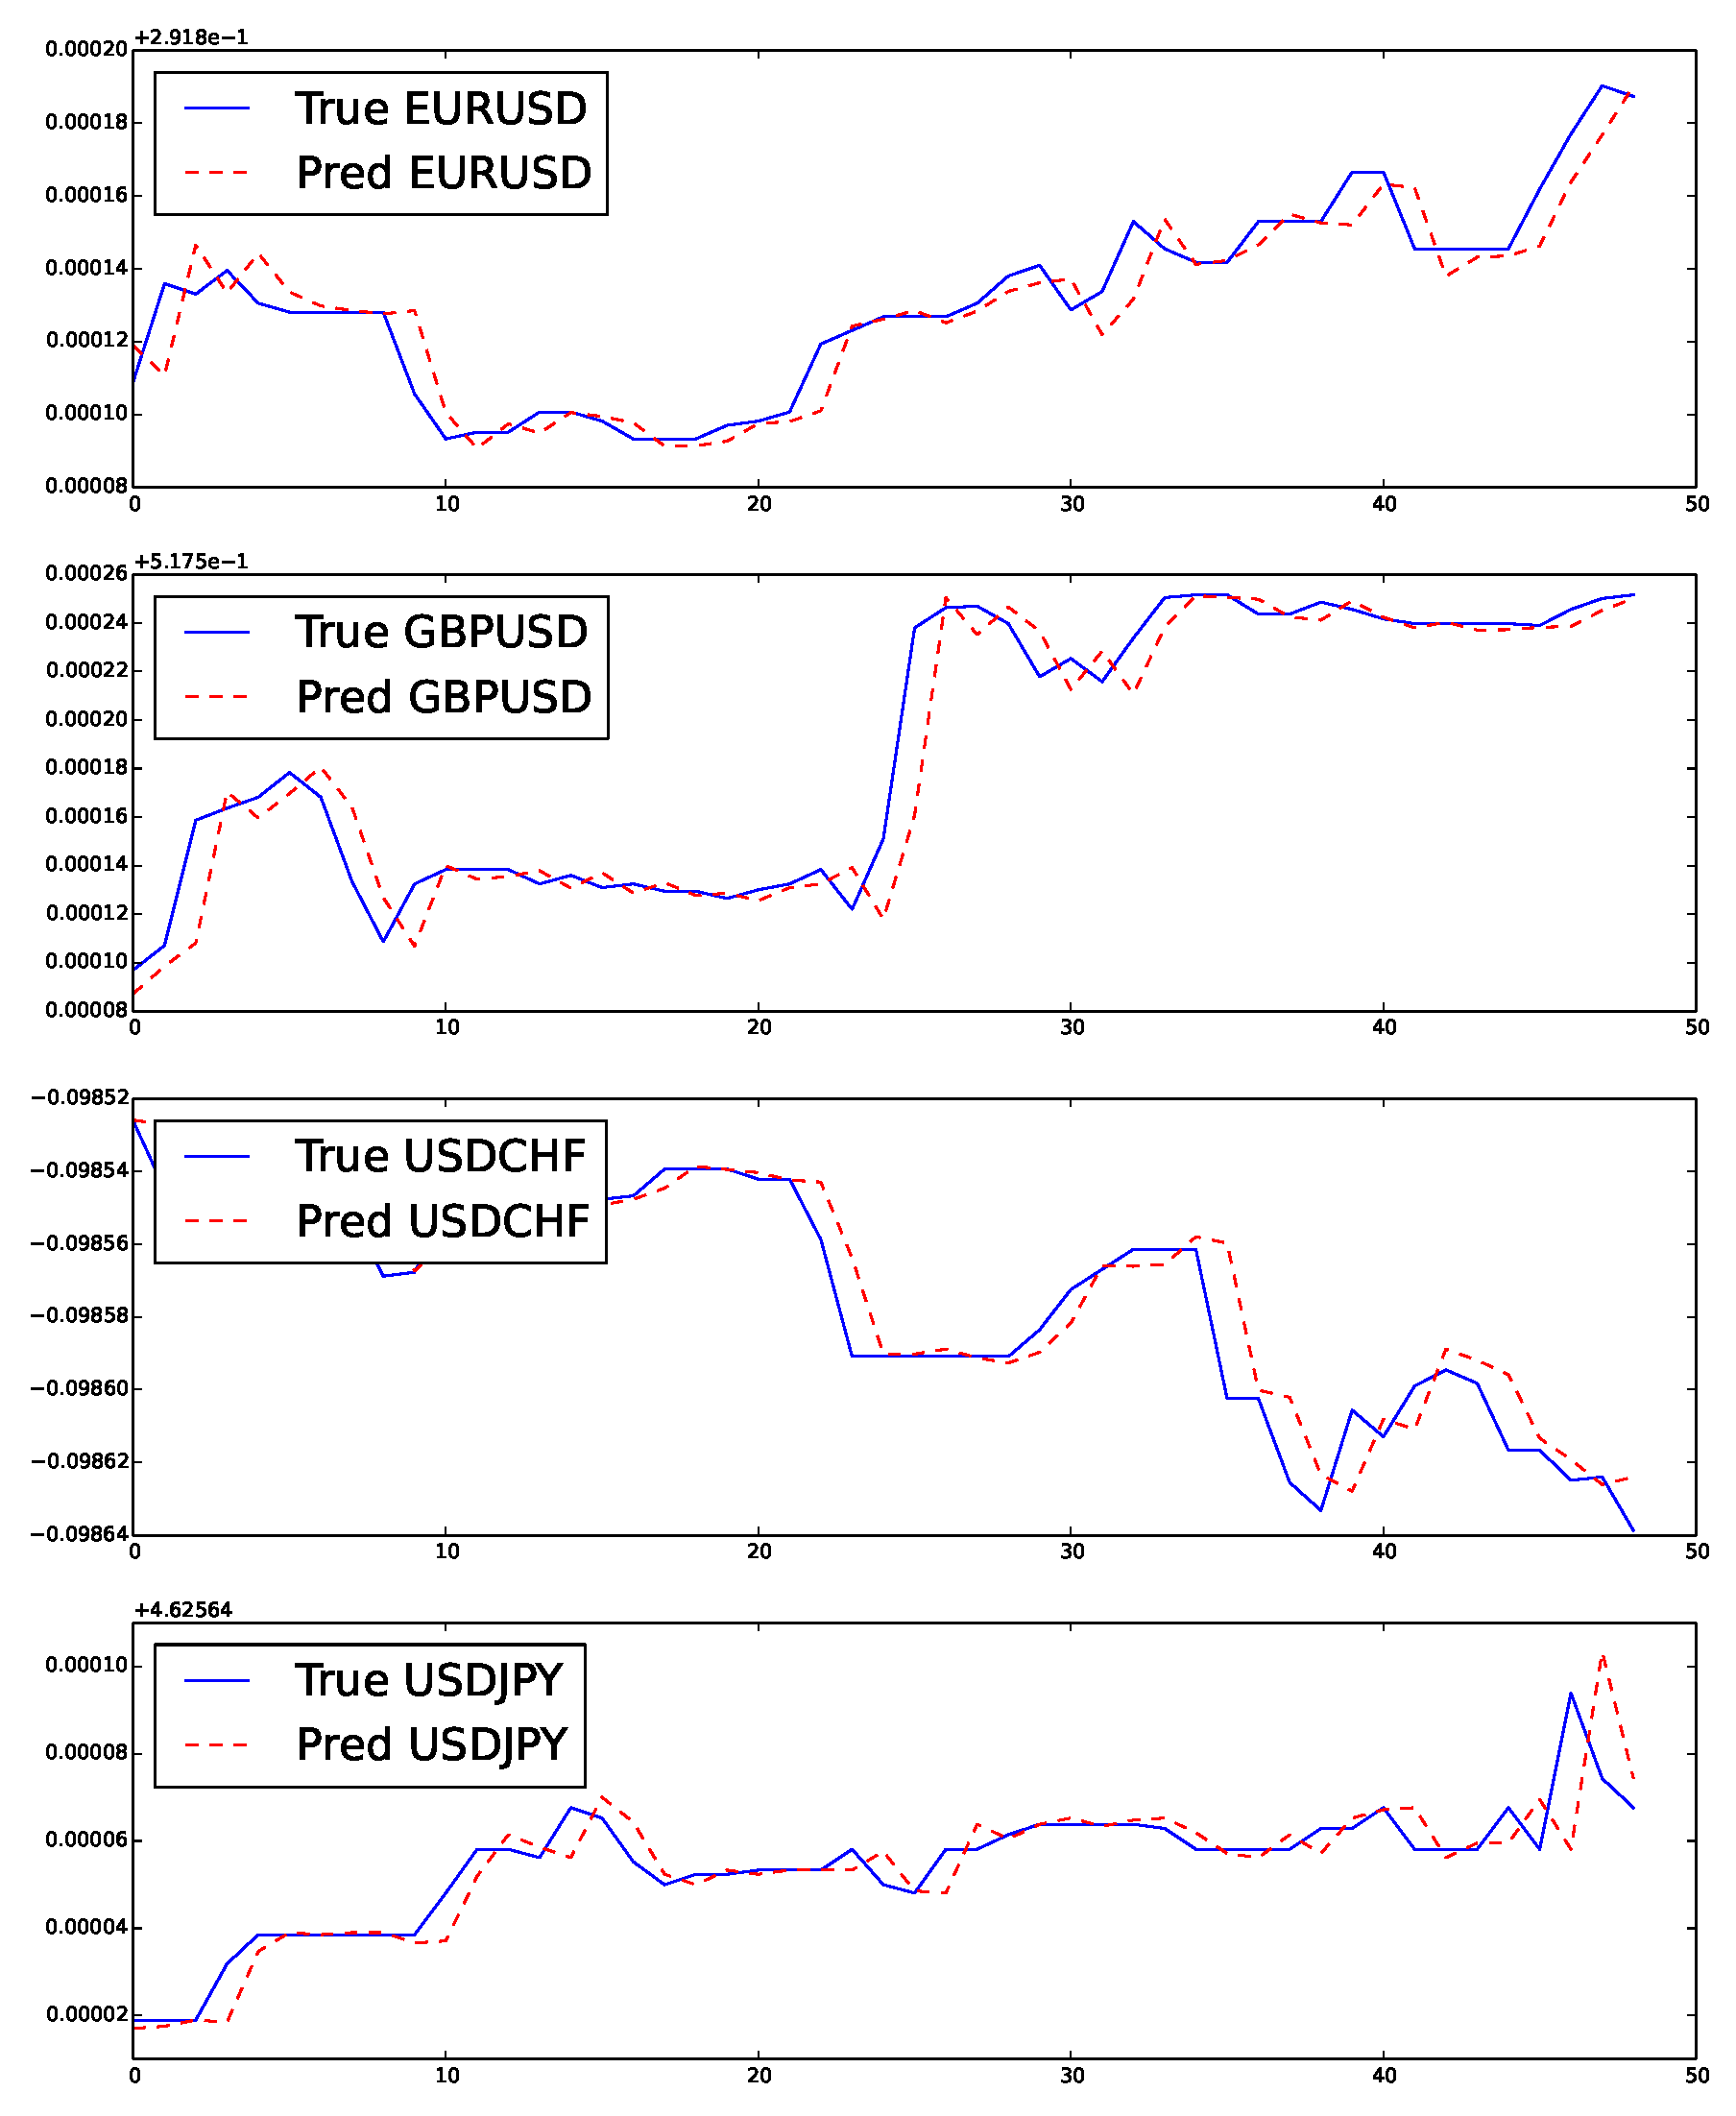
\epsfig{file = img/accuracy.eps, width = 7.5cm}}
%  \caption{Time series differences accuracy.}
%  \label{fig:accuracy}
% \end{figure}
%
%\begin{figure}[!h]
%  \vspace{-0.2cm}
%  \centering
%   {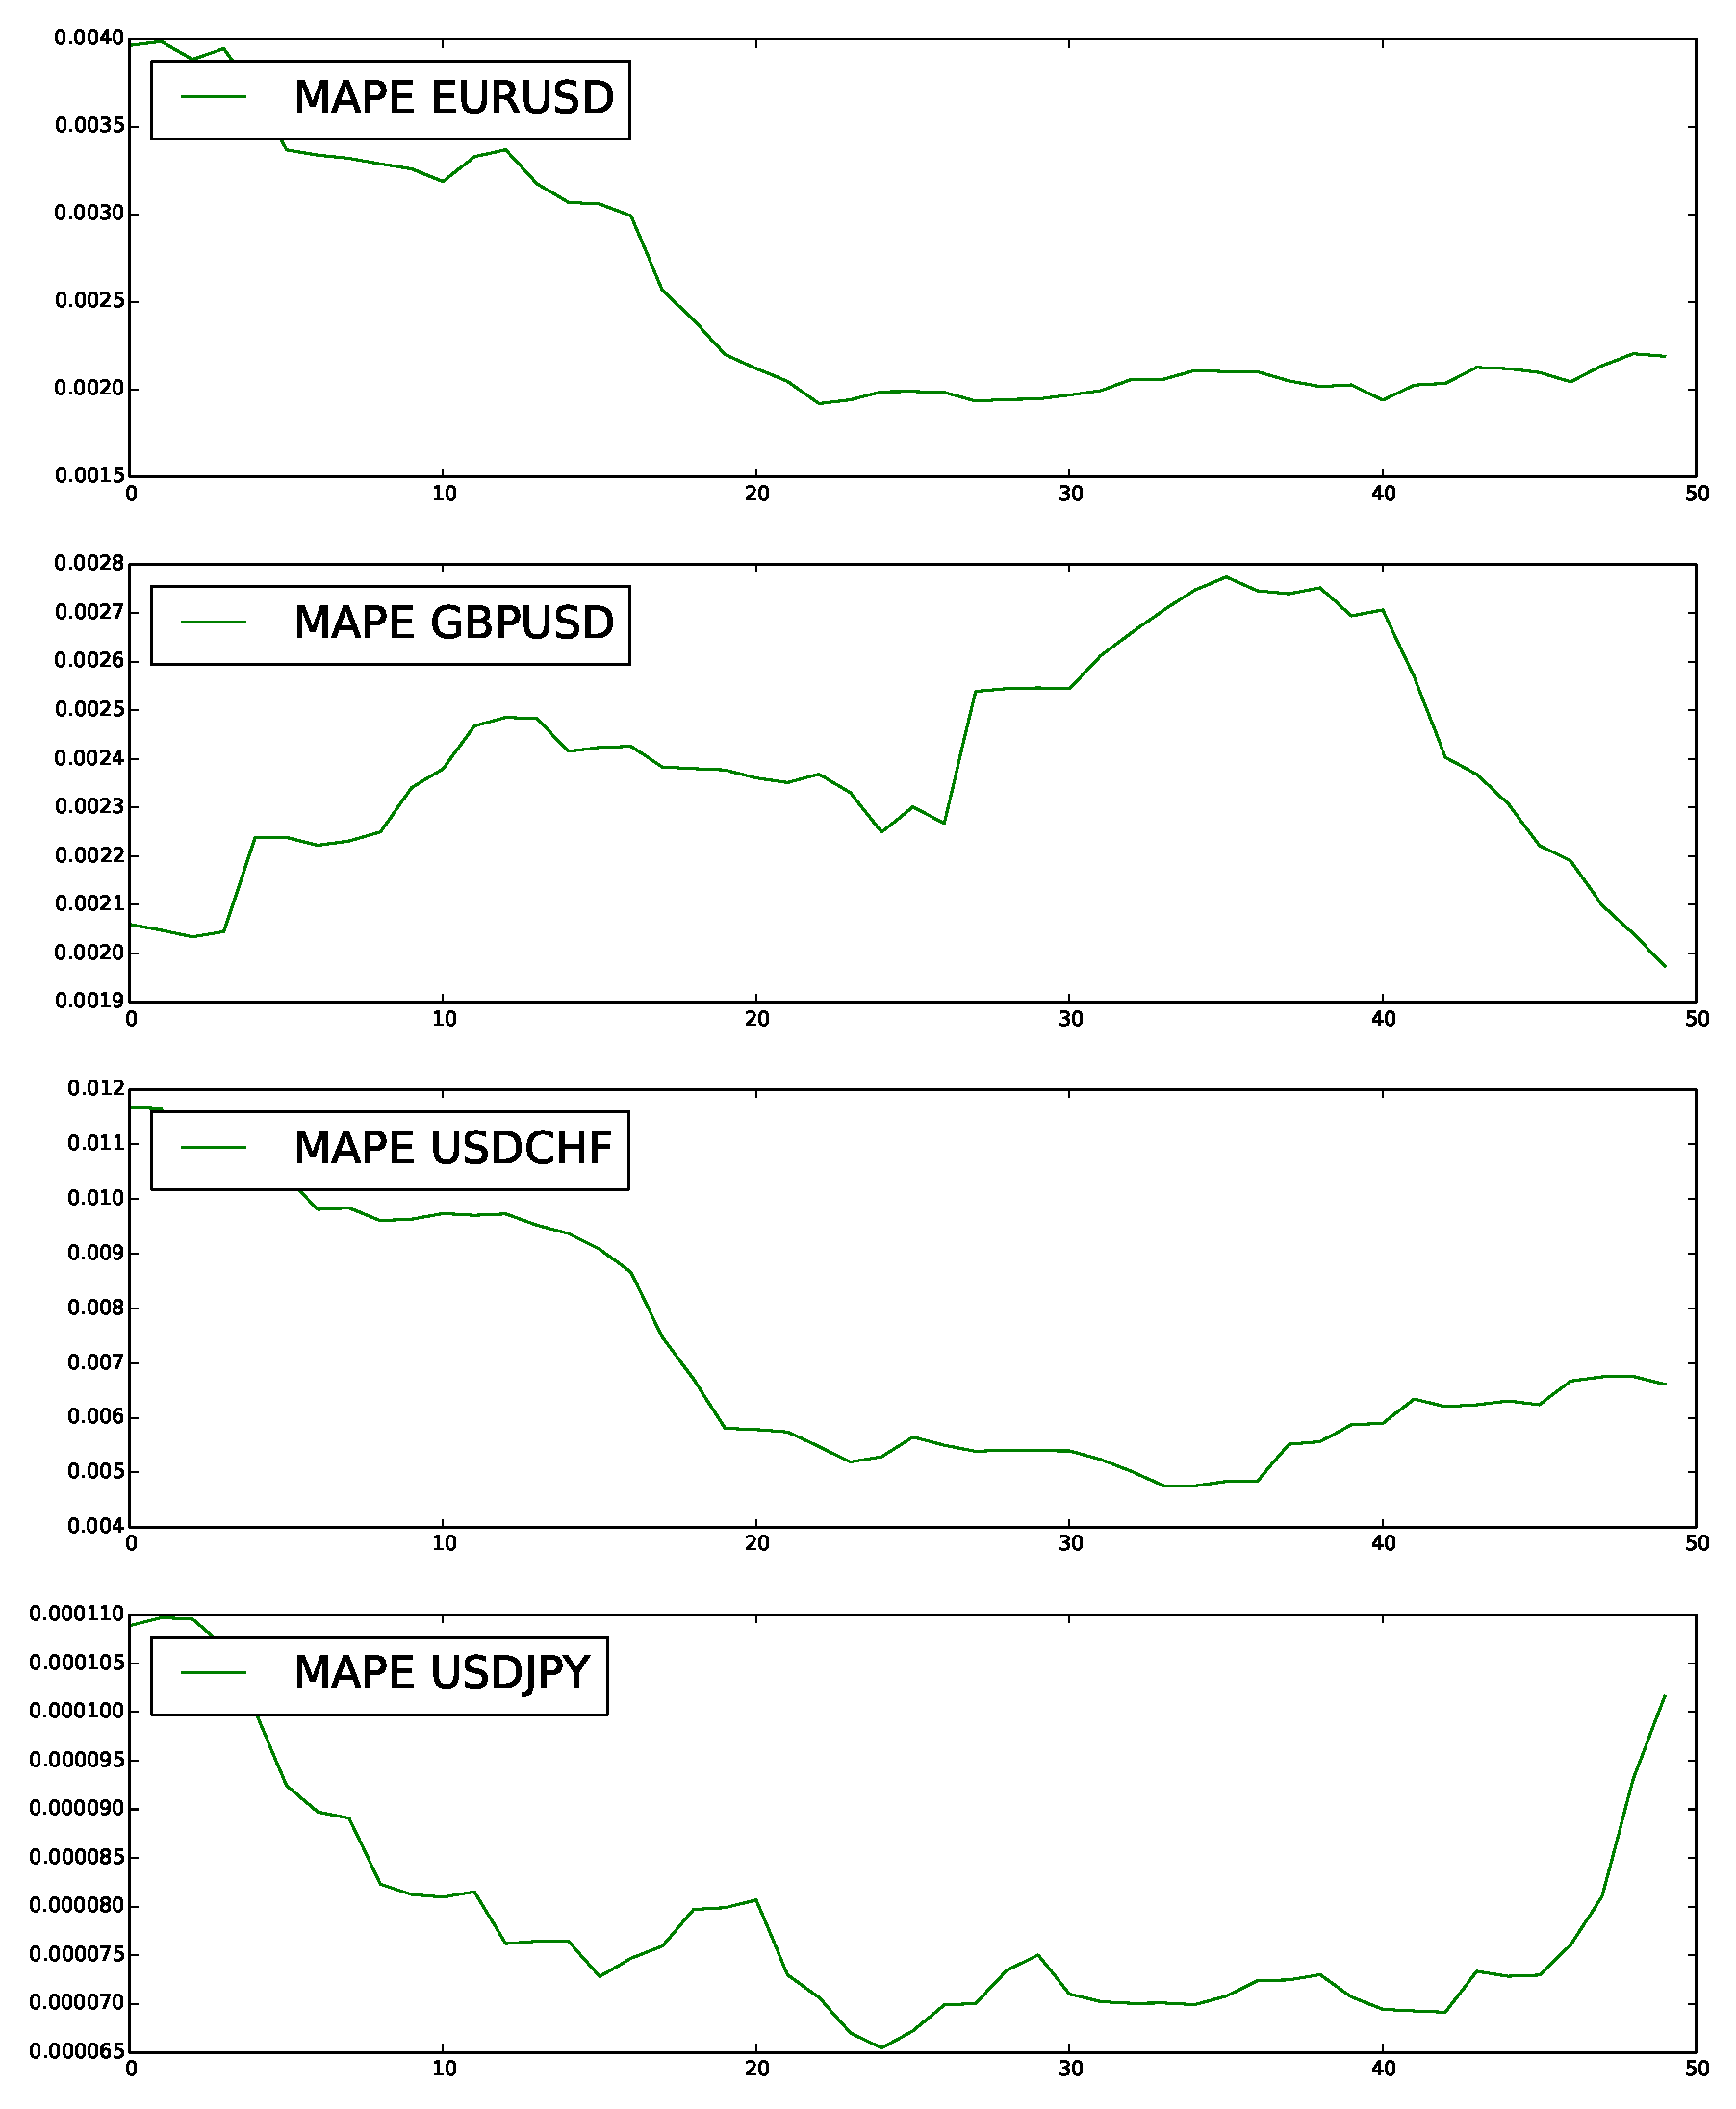
\epsfig{file = img/mapes.eps, width = 7.5cm}}
%  \caption{In-sample MAPEs example.}
%  \label{fig:mapes}
% \end{figure}

Despite the fact that MAPEs are high, figure ~\ref{fig:accuracy} shows some of
the out-of-sample forecasts made by our proposal OVECM which appears to follow
time series differences. 


\section{\uppercase{Conclusions}}
\label{sec:conclusions}
\noindent A new online vector error correction method was presented. The traditional VECM
was modified in order to use it in an online context. We have shown that our
proposed OVECM considerably reduces execution times without compromising
solution accuracy.  However the execution time of OVECM is only better than
SLVECM if we avoid the cointegration vector calculation using the Johansen
method, this is given by the avg\_error variable which controls how many times
the method is called.  We could see that our algorithm took much less than a
minute at every step. This means that it could also be used with higher
frequency data and would still provide responses before new data arrives. 
In all the presented scenarios, MAPE is still very high and for future
study, it would be interesting to improve the out-of-sample forecast by
considering more explicative variables, optimizing the windows size, the
number of lags or trying new condition to obtain new cointegration vectors.
Since OVECM is an online algorithm which optimizes processing time, it could be
used by investors as an input for strategy robots. Moreover, some technical
analysis methods could be based on its output. 



\vfill
\bibliographystyle{apalike}
{\small
\bibliography{reference}}

\vfill
\end{document}

